\chapter{Johnson-Rauschen}
% ----
In diesem Kapitel wird das Johnson-Rauschen in Widerständen untersucht.\\ 
Das Johnson-Rauschen entsteht durch die thermische Fluktuation der Ladungsträger in einem ohmschen Widerstand und führt zu zufälligen Spannungsschwankungen über dem Widerstand. Diese Spannungsschwankungen sind proportional zum Widerstand $R$, sowie seiner Temperatur $T$ und werden durch die Nyquist-Beziehung\cite{paper} beschrieben:
\begin{equation}
    \langle V^2 \rangle = 4 k_B T R \Delta f,
\end{equation}
wobei $\langle V^2 \rangle$ die mittlere quadratische (MS \enquote{mean square}) Spannung, $k_B$ die Boltzmann-Konstante und $\Delta f$ die effektive Bandbreite des Messsystems ist.
% ----
\section{Visualisierung des Johnson-Rauschens}
% ----
Zunächst wird das Johnson-Rauschen visuell dargestellt. Da es nur eine sehr geringe Signalstärke aufweist, wird das Rauschsignal mit einem speziellen Vorverstärker (\cref{fig:johnson_lle}), einem nicht-invertierenden Operationsverstärker eingebaut in die \enquote{\texttt{Low-Level electronics}-Box} (LLE), verstärkt. \\
\begin{figure}[h]
    \centering
    \subcaptionbox{Vorverstärker der LLE-Box}{\includegraphics[keepaspectratio, width=5cm]{figs/schalt_amplifier.png}}
    \subcaptionbox{LLE-Box}{\includegraphics[keepaspectratio, width=7cm]{figs/johnson_lle.png}}
    \caption{Schaltpläne zur Verstärkung des Johnson-Rauschens~\cite{praktikum4_atome}}\label{fig:johnson_lle}
\end{figure}

Die Verstärkerelektronik besteht aus zwei Stufen, sodass eine Gesamtverstärkung von $G_1 = 600$ erreicht wird. Das verstärkte Rauschsignal gelangt hiernach an die HLE-Box, einem Bandpass welcher gezielt die relevanten Frequenzbereiche herausfiltert und einem einstellbaren Verstärker (\enquote{Gain}), und wird schließlich auf dem Oszilloskop dargestellt (\cref{fig:johnson_aufbau}).
\begin{figure}[h]
    \centering
    \subcaptionbox{Schaltplan zur Messung des \\ Johnson-Rauschens~\cite{praktikum4_atome}}{\includegraphics[keepaspectratio,width=0.48\textwidth]{figs/johnson_hle.png}}
    \subcaptionbox{Johnson-Rauschen bei $T = \qty{21.4\pm 0.2}{\degreeCelsius}$;\\ $T$/div$=\qty{500}{\micro\second}$; $V$ / div $=\qty{800}{\milli\volt}$;\\ Triggerlevel $\approx 0$; Eingangsimpedanz am Oszilloskop:$\qty{1}{\mega\ohm}$}{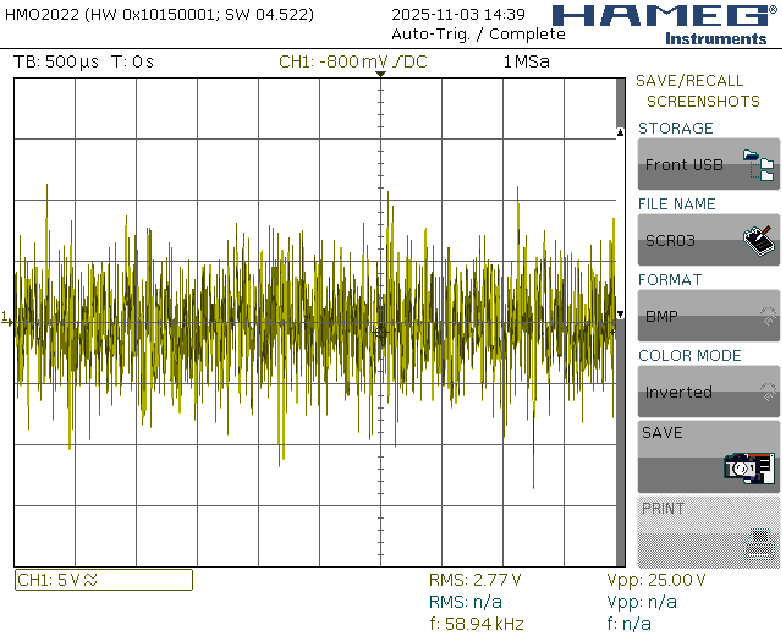
\includegraphics[keepaspectratio,width=0.48\textwidth]{images/johnson_oszi.pdf}}
    \caption{Visualisierung des Johnson-Rauschens}\label{fig:johnson_aufbau}
\end{figure}
\subsection{Beobachtung des Johnson-Rauschens}
Die Widerstände der LLE-Box werden auf $R_{\mathrm{in}} = \qty{100}{\kilo\ohm}$ und $R_f = \qty{1}{\kilo\ohm}$ und die Grenzfrequenzen der HLE-Box auf $f_{\mathrm{LP}} = \qty{10}{\kilo\hertz}$ und $f_{\mathrm{HP}} = \qty{1}{\kilo\hertz}$ eingestellt.\cite{praktikum4_atome}\\
Auf dem Oszilloskop ist das Rauschsignal als zufällige Spannungsschwankungen um den Mittelwert von Null zu erkennen (\cref{fig:johnson_aufbau}).
% ----
 \subsection{Messung des Johnson-Rauschens mit der HLE-Box}
% ----
Nun wird die HLE-Box wie in \cref{fig:johnson_hle_messung} an einen Multiplier im \emph{AxA}-Modus geschlossen.\\
Hierbei wird das Rauschsignal am Ausgang der HLE-Box gemäß
\begin{equation}
    V_{\mathrm{out}} = \frac{\overline{V_{\mathrm{in}}^2(t)}}{\qty{10}{\volt}}
\end{equation}
quadriert. Das Ausgangssignal des Multipliers wird intern durchgeschleift und über eine einstellbare Zeitkonstante $\tau=\qty{1}{\second}$ gemittelt. 
\begin{figure}[h]
    \centering
    \includegraphics[width=0.6\textwidth]{figs/johnson_hle_and_dmm.png}
    \caption{Schaltplan zur Messung des Johnson-Rauschens mit der HLE-Box~\cite{praktikum4_atome}}\label{fig:johnson_hle_messung}
\end{figure}